\documentclass[11pt,a4paper]{article}
\usepackage[utf8]{inputenc}
\usepackage[T1]{fontenc}
\usepackage{tgpagella}
\usepackage[spanish]{babel}
\usepackage{geometry}
\usepackage{booktabs}
\usepackage{xcolor}
\usepackage{titlesec}
\usepackage{fancyhdr}
\usepackage[parfill]{parskip}
\usepackage[expansion=false]{microtype}
\usepackage{hyperref}
\usepackage{setspace}
\usepackage{needspace}
\usepackage{graphicx}
\widowpenalty=10000
\clubpenalty=10000
\displaywidowpenalty=10000

\geometry{top=3.0cm,bottom=3.0cm,left=3.5cm,right=3.5cm}
\setlength{\parskip}{0.65em}
\setlength{\parindent}{0em}

\definecolor{azulai}{RGB}{30,80,140}
\definecolor{doradoai}{RGB}{140,90,0}
\definecolor{grisai}{RGB}{70,70,70}

\titleformat{\section}{\Large\bfseries\color{azulai}}{}{0em}{}[{\color{azulai}\titlerule[0.5pt]}]
\titlespacing*{\section}{0pt}{1.8em}{0.8em}
\titleformat{\subsection}{\large\bfseries\color{doradoai}}{}{0em}{}
\titlespacing*{\subsection}{0pt}{1.4em}{0.5em}
\titleformat{\subsubsection}{\normalsize\bfseries\color{grisai}}{}{0em}{}
\titlespacing*{\subsubsection}{0pt}{1.0em}{0.3em}

\pagestyle{fancy}\fancyhf{}
\rhead{\textcolor{grisai}{\small Amaya Beatriz — Arquitectura Interna}}
\lhead{\textcolor{grisai}{\small Júpiter · Saturno}}
\cfoot{\textcolor{grisai}{\small\thepage}}
\renewcommand{\headrulewidth}{0.3pt}

\hypersetup{colorlinks=true,linkcolor=azulai,urlcolor=azulai}
\setstretch{1.45}
\tolerance=1500
\emergencystretch=4em

\begin{document}

% ── Portada ──────────────────────────────────────────────────────────────────

\begin{titlepage}
\centering

\vspace*{2cm}

{\Huge\bfseries\color{azulai} Júpiter · Saturno}\\[0.4cm]

{\large\color{grisai} Arquitectura Interna}\\[0.25cm]

{\small\itshape\color{grisai}
Crecimiento, estructura y organización interna
}\\[1.8cm]

{\huge\color{doradoai} Amaya Beatriz}\\[1.2cm]

{\Large 30/10/1976 \quad 22:10}\\[0.25cm]

{\Large Zaragoza, España}\\[0.25cm]

{\normalsize
Lat: 41.6916° \quad
Lon: -0.9101° \quad
UTC+01:00
}\\[0.4cm]

{\normalsize
Ascendente: Cáncer 16°08'
\quad
MC: Piscis 25°32'
}\\[1.6cm]

\begin{tabular}{ll}
\textbf{Júpiter:} & Tauro — Casa 11 28°32' (Retrógrado) \\
\textbf{Saturno:} & Leo — Casa 2 16°10' \\
\end{tabular}

\vfill

{\small\color{grisai}
Generado el 19/05/2026
}

\end{titlepage}

	ableofcontents
space{0.8cm}

% ── Datos de referencia ──────────────────────────────────────────────────────

\section{Datos de referencia}

\begin{center}
\begin{tabular}{llll}
\toprule
\textbf{Punto} & \textbf{Signo} & \textbf{Casa} & \textbf{Posición} \\
\midrule

Júpiter (Retrógrado) &
Tauro &
Casa 11 &
28°32' \\

Saturno &
Leo &
Casa 2 &
16°10' \\

Sol &
Escorpio &
Casa 5 &
7°35' \\

Luna &
Acuario &
Casa 8 &
19°05' \\

Mercurio &
Escorpio &
Casa 5 &
2°48' \\

Venus &
Sagitario &
Casa 6 &
12°22' \\

Marte &
Escorpio &
Casa 5 &
15°07' \\

Urano &
Escorpio &
Casa 5 &
7°29' \\

Ascendente &
Cáncer &
--- &
16°08' \\

Medio Cielo &
Piscis &
--- &
25°32' \\

\bottomrule
\end{tabular}
\end{center}

\vspace{0.8cm}

\subsection*{Aspectos entre funciones}

\begin{center}
\begin{tabular}{lllll}
  \toprule
  \textbf{Planeta 1} & \textbf{Asp.} & \textbf{Planeta 2} & \textbf{Tipo} & \textbf{Orbe} \\
  \midrule
  Saturno & cua & Marte & Cuadratura & 1.0° \\
  Saturno & opo & Luna & Oposición & 2.9° \\
  Saturno & tri & Venus & Trígono & 3.8° \\
  \bottomrule
\end{tabular}
\end{center}

\vspace{1cm}

\begin{center}
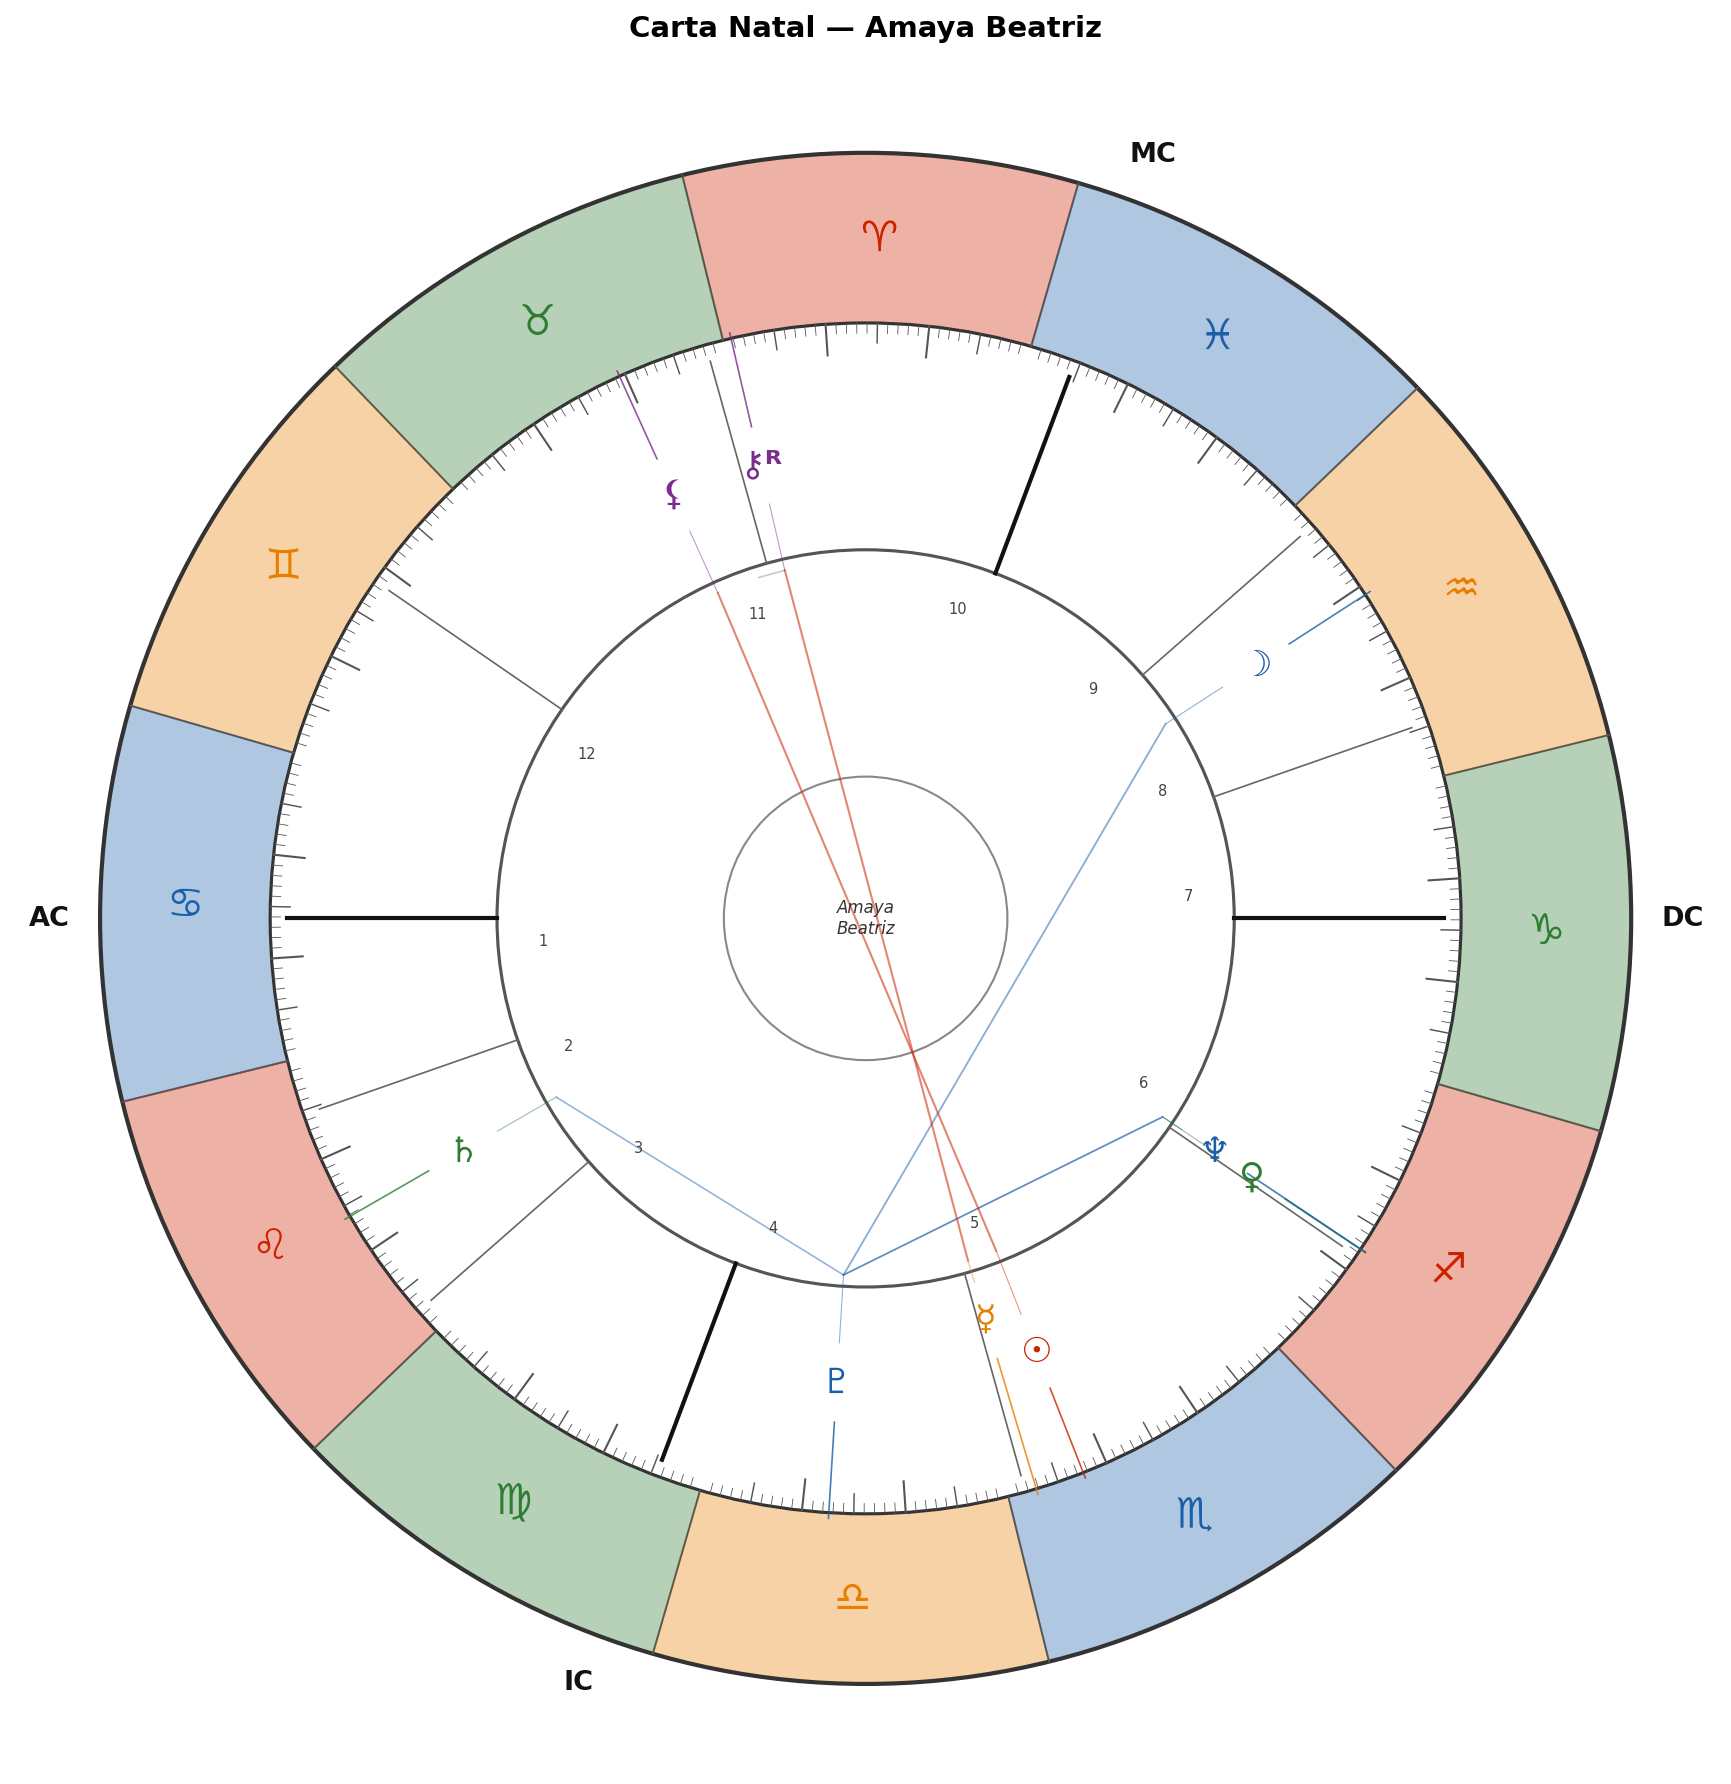
\includegraphics[width=0.72\textwidth]{Amaya_Beatriz_rueda.png}
\end{center}

\vspace{0.8cm}
\Needspace{5\baselineskip}


% ── Interpretación ───────────────────────────────────────────────────────────

\section{Interpretación — Arquitectura Interna}

\begin{center}
{\small\itshape
No se trata de definir quién eres.\\
Se trata de observar cómo tiendes a crecer, estructurarte\\
y sostener tu relación con el mundo.
}
\end{center}

\vspace{0.8cm}
\Needspace{5\baselineskip}

% ── 1. Estructura general ────────────────────────────────────────────────────

\subsection{1. Estructura general}

Júpiter está en Tauro, Casa 11: muestra cómo tiendes a crecer, abrir posibilidades y ampliar tu relación con el mundo.
Saturno está en Leo, Casa 2: muestra cómo tiendes a estructurarte, sostener límites y construir estabilidad.

Expansión (Tauro, Tierra) y estructura (Leo, Fuego) operan en elementos que crean tensión. Puede haber momentos en los que crecer y sostenerte requieran movimientos internos diferentes, por lo que la integración necesita más atención consciente.

Aspectos relevantes: Saturno–Luna en oposición (orbe 2.92°), Saturno–Venus en trígono (orbe 3.8°), Saturno–Marte en cuadratura (orbe 1.04°).

\vspace{0.8cm}
\Needspace{5\baselineskip}

% ── 2. Júpiter ───────────────────────────────────────────────────────────────

\subsection{2. Júpiter — Expansión y crecimiento}

\subsubsection*{
Júpiter en Tauro
— Casa 11 (Retrógrado)
}

Tiendes a crecer consolidando, estabilizando y profundizando en lo que ya existe. La expansión aparece cuando puedes construir algo sólido, útil y sostenible en el tiempo. Necesitas sentir continuidad y cierta seguridad para avanzar.

En situaciones de desbordamiento: puedes aferrarte demasiado a estructuras, vínculos o formas de funcionamiento que ya han cumplido su ciclo. La necesidad de conservar dificulta hacer espacio para lo nuevo. En momentos de estancamiento: puedes necesitar demasiadas garantías antes de dar un paso importante. El miedo a perder estabilidad puede retrasar movimientos necesarios.

Tiendes a crecer a través de grupos, redes y proyectos compartidos. La expansión aparece cuando puedes participar en algo colectivo y aportar tu visión a espacios más amplios que lo estrictamente personal. Necesitas conexión con ideas, personas o proyectos que miren hacia el futuro.

Júpiter está retrógrado. El crecimiento tiende a desarrollarse de forma más interna y menos visible externamente al principio. Puedes necesitar más tiempo para traducir expansión o comprensión en movimientos concretos hacia fuera.

\vspace{0.8cm}
\Needspace{5\baselineskip}

% ── 3. Saturno ───────────────────────────────────────────────────────────────

\subsection{3. Saturno — Estructura y sostén}

\subsubsection*{
Saturno en Leo
— Casa 2
}

Tiendes a estructurarte a través de la expresión sostenida y la construcción de una identidad coherente. Necesitas sentir continuidad entre lo que eres, lo que haces y la forma en que eso puede mostrarse al mundo. La estructura aparece desarrollando algo propio con consistencia.

El límite aparece cuando el reconocimiento externo no acompaña el esfuerzo que estás realizando. No siempre el entorno puede responder en la medida esperada.

Cuando la estructura deja de sostenerse: puedes aumentar demasiado el esfuerzo buscando validación o perder motivación si la respuesta externa desaparece. La dependencia del reconocimiento vuelve más frágil la estabilidad interna.

Tiendes a estructurarte a través de los recursos, la estabilidad y la gestión de lo que tiene valor para ti. La seguridad suele construirse lentamente, mediante constancia y acumulación progresiva. Necesitas sentir que existe una base concreta sobre la que apoyarte.

El límite aparece cuando intentas sostener más de lo que tus recursos reales permiten. La estabilidad depende de la capacidad de administrar energía, tiempo y recursos de forma sostenible.

Saturno oposición Luna: necesidad emocional y necesidad de estructura compiten entre sí. Cuando priorizas control, responsabilidad o estabilidad, puede costarte acceder a lo emocional. Cuando lo emocional ocupa más espacio, sostener estructura se vuelve más difícil.

Necesitas aprender cuándo contener y cuándo permitir mayor flexibilidad emocional.

\vspace{0.8cm}
\Needspace{5\baselineskip}

% ── 4. Integración ───────────────────────────────────────────────────────────

\subsection{4. Integración — Crecimiento y estructura}

Júpiter en Tauro (Tierra) y Saturno en Leo (Fuego) no forman aspecto directo, pero operan en elementos que crean tensión. Esto puede hacer que crecer y sostenerte requieran movimientos internos diferentes. La expansión y la estructura no se alimentan de forma automática; necesitas integrarlas de manera consciente para no abrir posibilidades sin sostén ni construir estructuras sin crecimiento real.

Cuando Júpiter domina: puedes acumular más de lo que puedes gestionar, generando peso sin avance real. La estructura de Saturno en Leo no compensa con suficiente rapidez y lo que ganas en amplitud empieza a perder forma.

Cuando Saturno domina: la acción puede frenarse antes de producir resultado y la vitalidad queda contenida demasiado pronto. La expansión de Júpiter en Tauro no encuentra espacio para activarse y puedes mantener lo que ya existe sin crecer hacia lo que sería posible.

Bajo presión suele aparecer una secuencia bastante reconocible. Primero, Saturno en Leo empieza a ceder: el ritmo de acción supera la capacidad real de organización. Después, Júpiter en Tauro ocupa ese espacio: acumulas carga, tareas o responsabilidades sin que exista una estructura clara que las sostenga. Desde ahí puedes intentar recuperar estabilidad rápidamente, pero lo que construyes en ese estado suele ser más rígido, reactivo o agotador de sostener. Si el patrón no se reconoce a tiempo, el ciclo tiende a repetirse.

\vspace{0.8cm}
\Needspace{5\baselineskip}

% ── 5. Orientación práctica ──────────────────────────────────────────────────

\subsection{5. Orientación práctica}

\subsubsection*{Desde dónde empezar}

El punto de entrada más accesible suele estar en la estructura (Leo, Casa 2). De las dos funciones, esta requiere menos resistencia para activarse. La forma más natural de empezar es activar movimiento antes de tener todo completamente resuelto. Cuando todo parece bloqueado, comenzar por aquí suele facilitar que la otra función también pueda ponerse en marcha.

\subsubsection*{Qué sostener}

Lo más importante de sostener aparece en Saturno (Leo, Casa 2). Bajo presión puedes abrir posibilidades o reaccionar antes de mantener forma estable. Conviene cuidar especialmente recordar el objetivo que da sentido al esfuerzo. Muchas veces la primera señal de desgaste aparece cuando sigues haciendo cosas, pero ya no existe suficiente estructura para sostenerlas bien.

\subsubsection*{Qué evitar}

Conviene evitar que la función más activa en cada momento desplace completamente a la otra. Con Júpiter en Tauro (Tierra) y Saturno en Leo (Fuego), crecimiento y estructura no se activan automáticamente juntos. Necesitas reconocer conscientemente cuándo hace falta abrir más espacio y cuándo hace falta construir más sostén.

\subsubsection*{Si no se integra}

Cuando crecimiento y estructura dejan de colaborar, puede aparecer expansión sin suficiente sostén o estabilidad sin movimiento real. En ambos casos se pierde parte de lo que realmente podría desarrollarse si ambas funciones trabajaran en la misma dirección.

\subsubsection*{Señal temprana}

La primera señal suele aparecer en Saturno (Leo): el ritmo aumenta más rápido que la capacidad de consolidar. Cuando eso ocurre, Júpiter (Tauro) tiende a ocupar rápidamente el espacio disponible y la expansión puede acelerarse más de lo que realmente puedes sostener. Detectar la señal temprano suele evitar entrar en ciclos más agotadores.

\vfill

\begin{center}
{\small\itshape\color{grisai}
La astrología se utiliza aquí como herramienta simbólica de observación\\
y no como una definición cerrada de la persona.
}
\end{center}

\end{document}
